\documentclass{article}
\usepackage[utf8]{inputenc}
\usepackage[T1]{fontenc}
\usepackage{ amssymb }
\usepackage{amsmath}
\usepackage{graphicx}

\title{Compiler Construction Problem Set 1}
\author{Magnus Brevik}
\date{January 2023}

\begin{document}
\noindent
\maketitle

\section{Regular languages, NFAs and DFAs}
\subsection{}
$\mathcal{L}$(a?a?(ba?a?)*)

\subsection{}
Not including a graph as this should be sufficient to replicate one. \\
State 0 is the starting state. \\
State 5 is the accepting state.
\begin{flalign*}
\textbf{State}&\qquad&\textbf{Letter}&\qquad&\textbf{Result State}&\qquad\qquad\qquad\qquad\qquad\qquad\qquad&\\
0:&&a&&1&&\\
&&\epsilon&&1&&\\
1:&&a&&2&&\\
&&\epsilon&&2&&\\
2:&&b&&3&&\\
&&\epsilon&&5&&\\
3:&&a&&4&&\\
&&\epsilon&&4&&\\
4:&&a&&5&&\\
&&\epsilon&&5&&\\
5:&&\epsilon&&2&&
\end{flalign*}

\pagebreak

\subsection{}
DFA State 0 is the start state. \\
Accepting DFA States are \{0, 1, 2, 3, 4\}\\
State 5 is a dead end.
\begin{flalign*}
\textbf{DFA State}&\qquad&&\textbf{NFA States}&\qquad\qquad\qquad\qquad\qquad\qquad\qquad&\\
0&&&\{0, 1, 2, 5\}\\
1&&&\{1, 2, 5\}\\
2&&&\{2, 3, 4, 5\}\\
3&&&\{2, 4, 5\}\\
4&&&\{2, 5\}\\
5&&&\{\}
\end{flalign*}
\textbf{Rules:}
\begin{flalign*}
\textbf{State}&\qquad&\textbf{Letter}&\qquad&\textbf{Result State}&\qquad\qquad\qquad\qquad\qquad\qquad\qquad&\\
0:&&a&&1&&\\
&&b&&2&&\\
1:&&a&&4&&\\
&&b&&2&&\\
2:&&a&&3&&\\
&&b&&2&&\\
3:&&a&&4&&\\
&&b&&2&&\\
4:&&a&&5&&\\
&&b&&2&&\\
5:&&a|b&&5&&
\end{flalign*}

\pagebreak

\subsection{}
I forgot my crayons at home, so instead of colours I will use a letter with a subscript number for the intermediate states during minimisation. \\
Accepting States ($a_0$): \{0, 1, 2, 3, 4\} \\
Non-accepting States ($a_1$): \{5\} \\
\begin{flalign*}
    \qquad \text{Non-minimal State:}&\quad&0&\qquad&1&\qquad&2&\qquad&3&\qquad&4&\qquad&5&\qquad\\
    a:&&a_0&&a_0&&a_0&&a_0&&a_1&&a_1&\\
    b:&&a_0&&a_0&&a_0&&a_0&&a_0&&a_1&\\
\end{flalign*}
States \{0, 1, 2, 3\} are identical within group $a_0$, while 4 is different.\\
Next step uses the groups
\begin{flalign*}
    \qquad b_0:&\quad\{0,1,2,3\}&\qquad \\
    b_1:&\quad\{4\}&\\
    b_2:&\quad\{5\}&
\end{flalign*}
\begin{flalign*}
    \qquad \text{Non-minimal State:}&\quad&0&\qquad&1&\qquad&2&\qquad&3&\qquad&4&\qquad&5&\qquad\\
    a:&&b_0&&b_1&&b_0&&b_1&&b_2&&b_2&\\
    b:&&b_0&&b_0&&b_0&&b_0&&b_0&&b_1&\\
\end{flalign*}
States \{0, 2\} and \{1, 3\} are identical within group $b_0$.\\
Next step uses the groups
\begin{flalign*}
    \qquad c_0:&\quad\{0,2\}&\qquad \\
    c_1:&\quad\{1,3\}&\\
    c_2:&\quad\{4\}&\\
    c_3:&\quad\{5\}&
\end{flalign*}
\begin{flalign*}
    \qquad \text{Non-minimal State:}&\quad&0&\qquad&1&\qquad&2&\qquad&3&\qquad&4&\qquad&5&\qquad\\
    a:&&c_1&&c_2&&c_1&&c_2&&c_3&&c_3&\\
    b:&&c_0&&c_0&&c_0&&c_0&&c_0&&c_3&\\
\end{flalign*}
Now all groups consist of only identical NFA states, therefore we can rename them to just the number from the intermediate state names, and get
\begin{flalign*}
    \qquad 0:&\quad\{0,2\}&\qquad \\
    1:&\quad\{1,3\}&\\
    2:&\quad\{4\}&\\
    3:&\quad\{5\}&
\end{flalign*}
with the rules
\begin{flalign*}
    \textbf{State}&\qquad&\textbf{Letter}&\qquad&\textbf{Result State}&\qquad\qquad\qquad\qquad\qquad\qquad\qquad&\\
    0:&&a&&1&&\\
    &&b&&0&&\\
    1:&&a&&2&&\\
    &&b&&0&&\\
    2:&&a&&3&&\\
    &&b&&0&&\\
    3:&&a|b&&3&&
\end{flalign*}
where state 0 is the starting state, states \{0, 1, 2\} are accepting states, and state 5 is a dead end.

\subsection{}
To be honest I cannot find a good way to negate DFA without just going through the same steps of making a regular expression and following the same steps. 
I might just be missing something in the book or online about it, but did not find anything interesting when searching for "negate deterministic finite automaton". \\
Instead I made the regular expression (a|b)*aaa(a|b)* and made an automaton through NFA and NFA to DFA algorithms.\\
State 0 is the starting state, state 3 is the accepting state, and state 4 is a dead end.
\begin{flalign*}
    \textbf{State}&\qquad&\textbf{Letter}&\qquad&\textbf{Result State}&\qquad\qquad\qquad\qquad\qquad\qquad\qquad&\\
    0:&&a&&1&&\\
    &&b&&0&&\\
    1:&&a&&2&&\\
    &&b&&4&&\\
    2:&&a&&3&&\\
    &&b&&4&&\\
    3:&&a|b&&3&&\\
    4:&&a|b&&4&&
\end{flalign*}
I found inverting the regular expression easier, but this was also a very simple expression to just create without the original, which is what I actually did. There is probably some algorithm to invert or negate a DFA which I did not find which makes it easier than negating a regular expression.

\section{DFA for a small language}
\subsection{}
In modern regex one can usually use the identifier $\backslash$d to denote a digit, i.e. [0-9].\\
(d(x|y)=-?$\backslash$d+)|(go)$\backslash$n

\subsection{}
State 9 is the invalid state, so any invalid characters point there.\\
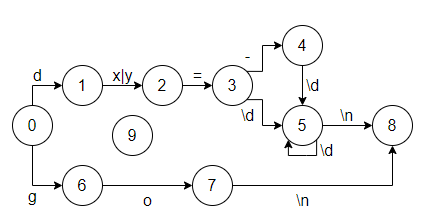
\includegraphics{grpah.png}
\subsection{}
Code implementation
\end{document}
